\documentclass[a4paper,12pt]{book}
\usepackage[utf8]{inputenc}
\usepackage{graphicx}
\usepackage{caption}
\usepackage{subcaption}
\graphicspath{ {./screen_shots/} }
\usepackage{hyperref}
\usepackage{float}

\begin{document}

\author{}
\title{MANUAL v0.30}
\date{\today}

\frontmatter
\maketitle
\tableofcontents

\mainmatter

\chapter{Difference to previous version}
Added section \ref{Georeferencing_with_WGS84toCartesian}: Georeferencing with WGS84toCartesian.

\chapter{Introduction}
This manual is prepared for mobile mapping system \url{https://github.com/JanuszBedkowski/mandeye_controller/blob/main/doc/manual/manual_v0_2/mandeye_dev_manual_v0_2.pdf}{MANDEYE} available as open hardware project.
The software is composed of:
\begin{itemize}
	\item Lidar odometry (for initial trajectory calculation),
	\item Multi view terrestrial laser scan registration (for final trajectory calculation).
\end{itemize}
To use the software click the link below:

\url{https://github.com/MapsHD/HDMapping/releases}
\linebreak
and download the latest version of files: laszip3.dll, \verb|lidar_odometry_step_1.exe|, \verb|multi_session_registration_step_3.exe|  and \verb|multi_view_tls_registration_step_2.exe|.
Then put all of the downloaded files in one folder and proceed to next chapter.





\chapter{Lidar odometry (step 1)}
This software calculates trajectory based on Lidar and IMU data.
It based on novel approach that I published in \url{https://www.softxjournal.com/article/S2352-7110(23)00314-X/pdf}.
Basically it is SAM (Smoothing and Mapping) approach that is using multi view Normal Distributions Transform in pose graph SLAM framework writen from scratch in Python (SymPy) and C++ (Eigen).
In Release v0.37 there is new option 'Consistency' that smooths the trajectory.
You can use it before saving data (please follow instructions in GUI).  
 

\begin{figure}
	\centering
	\includegraphics[width=\textwidth]{1.png}
	\caption{Step 1 - loading data.}
	\label{fig:1}
\end{figure}

\begin{figure}
	\centering
	\includegraphics[width=\textwidth]{2.png}
	\caption{Step 2 - select all *.csv and *.laz files from folder that \href{https://github.com/JanuszBedkowski/mandeye_controller/blob/main/doc/manual/manual_v0_1/mandeye_dev_manual_v0_1.pdf}{MANDEYE} mobile mapping system created on USB drive.}
	\label{fig:2}
\end{figure}

\begin{figure}
	\centering
	\includegraphics[width=\textwidth]{3.png}
	\caption{Step 3 - press 'compute all'. Check console mean time and folder 'preview'.}
	\label{fig:3}
\end{figure}

\begin{figure}
	\centering
	\includegraphics[width=\textwidth]{4.png}
	\caption{Optional step: intermediate results are stored in 'preview' folder.}
	\label{fig:4}
\end{figure}

\begin{figure}
	\centering
	\includegraphics[width=\textwidth]{5.png}
	\caption{Optional step: You can watch the progress in open source \href{https://www.cloudcompare.org/}{CloudCompare} software by loading all *.laz files from 'preview' folder.}
	\label{fig:5}
\end{figure}

\begin{figure}
	\centering
	\includegraphics[width=\textwidth]{6.png}
	\caption{Progress in console.}
	\label{fig:6}
\end{figure}

\begin{figure}
	\centering
	\includegraphics[width=\textwidth]{7.png}
	\caption{Final data in \href{https://www.cloudcompare.org/}{CloudCompare}.}
	\label{fig:7}
\end{figure}

\begin{figure}
	\centering
	\includegraphics[width=\textwidth]{8.png}
	\caption{Final data ready for export.}
	\label{fig:8}
\end{figure}

\begin{figure}
	\centering
	\includegraphics[width=\textwidth]{9.png}
	\caption{Exported final files.}
	\label{fig:9}
\end{figure}

\chapter{Multi view terrestrial laser scan registration (steps 2 and 3)}
\section{Step 2}
\begin{figure}[H]
	\centering
	\includegraphics[width=\textwidth]{10.png}
	\caption{Load session.json prepared by 'Lidar odometry'.}
	\label{fig:10}
\end{figure}

\begin{figure}[H]
	\centering
	\includegraphics[width=\textwidth]{13.png}
	\caption{Prepare field of view and change decimation to see more points. Generate random colors option is recommended for next steps as every scan will be in a different color.}
	\label{fig:13}
\end{figure}

\begin{figure}[H]
	\centering
	\includegraphics[width=\textwidth]{14.png}
	\caption{Turn on Manual Pose Graph Loop Closure Mod, then choose two different scans that share scanned objects, but difference in their numbers is as big as possible e.g. when you made a loop during scanning and came back to the same place after some time. Then click add edge.} 
	\label{fig:14}
\end{figure}

\begin{figure}[H]
	\centering
	\includegraphics[width=\textwidth]{15.png}
	\caption{Turn on manipulate active edge, turn on gizmo and align scan to scan manually.}
	\label{fig:15}
\end{figure}

\begin{figure}[H]
	\centering
	\includegraphics[width=\textwidth]{16.png}
	\caption{Once You are not capable of aligning more accurately, then turn off gizmo and repetitively use ICP until scans align to the level at which nothing can change anymore.}
	\label{fig:16}
\end{figure}

\begin{figure}[H]
	\centering
	\includegraphics[width=\textwidth]{17.png}
	\caption{Turn off manipulate active edge, click "set initial poses as motion model", then click "compute pose graph SLAM".}
	\label{fig:17}
\end{figure}

\begin{figure}[H]
	\centering
	\includegraphics[width=\textwidth]{18.png}
	\caption{Turn off Manual Pose Graph Loop Closure Mod and inspect if everything is ok, if not,  repeat steps from figures 3.3-3.6 (choose another pair of scans, refine them and compute the pose graph SLAM).}
	\label{fig:18}
\end{figure}

\begin{figure}[H]
	\centering
	\includegraphics[width=\textwidth]{19.png}
	\caption{Once the job is done click Save session button to save changes to session.json and export data to *.laz. The latter is Your map that can be loaded by e.g. \href{https://www.cloudcompare.org/}{CloudCompare}.}
	\label{fig:19}
\end{figure}
\pagebreak
{\large \textbf{Should a division of a session be needed, follow the steps below that describe how to do this in multi view tls registration step 2 program which is part of the HDMapping software:}}
\begin{figure}[H]
	\centering
	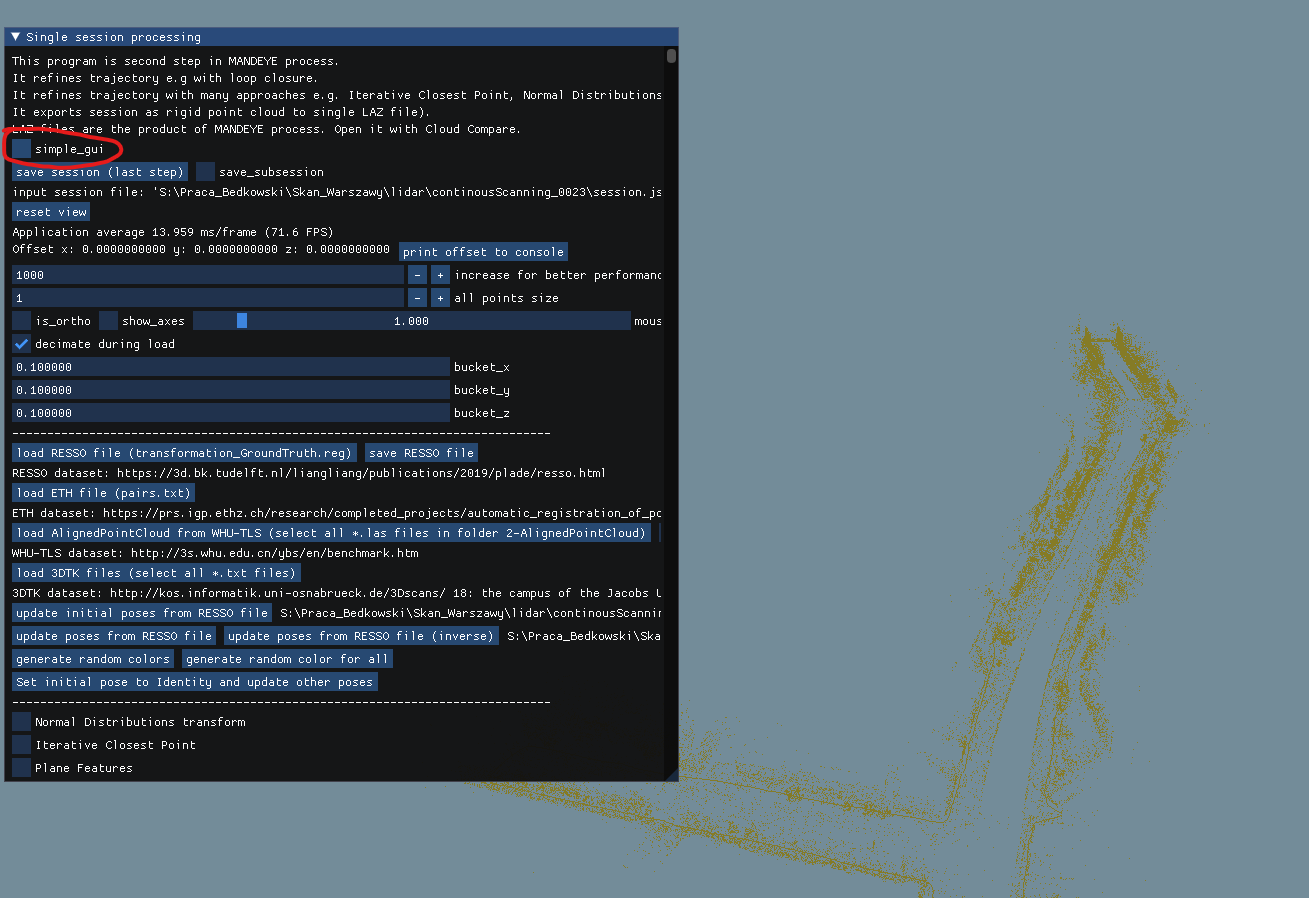
\includegraphics[width=\textwidth]{Cut_session1.png}
	\caption{Load the session as usual into step 2, prepare boundary scan numbers that will outline parts of scans, when prepared toggle off the simple gui.}
	\label{fig:20}
\end{figure}

\begin{figure}[H]
	\centering
	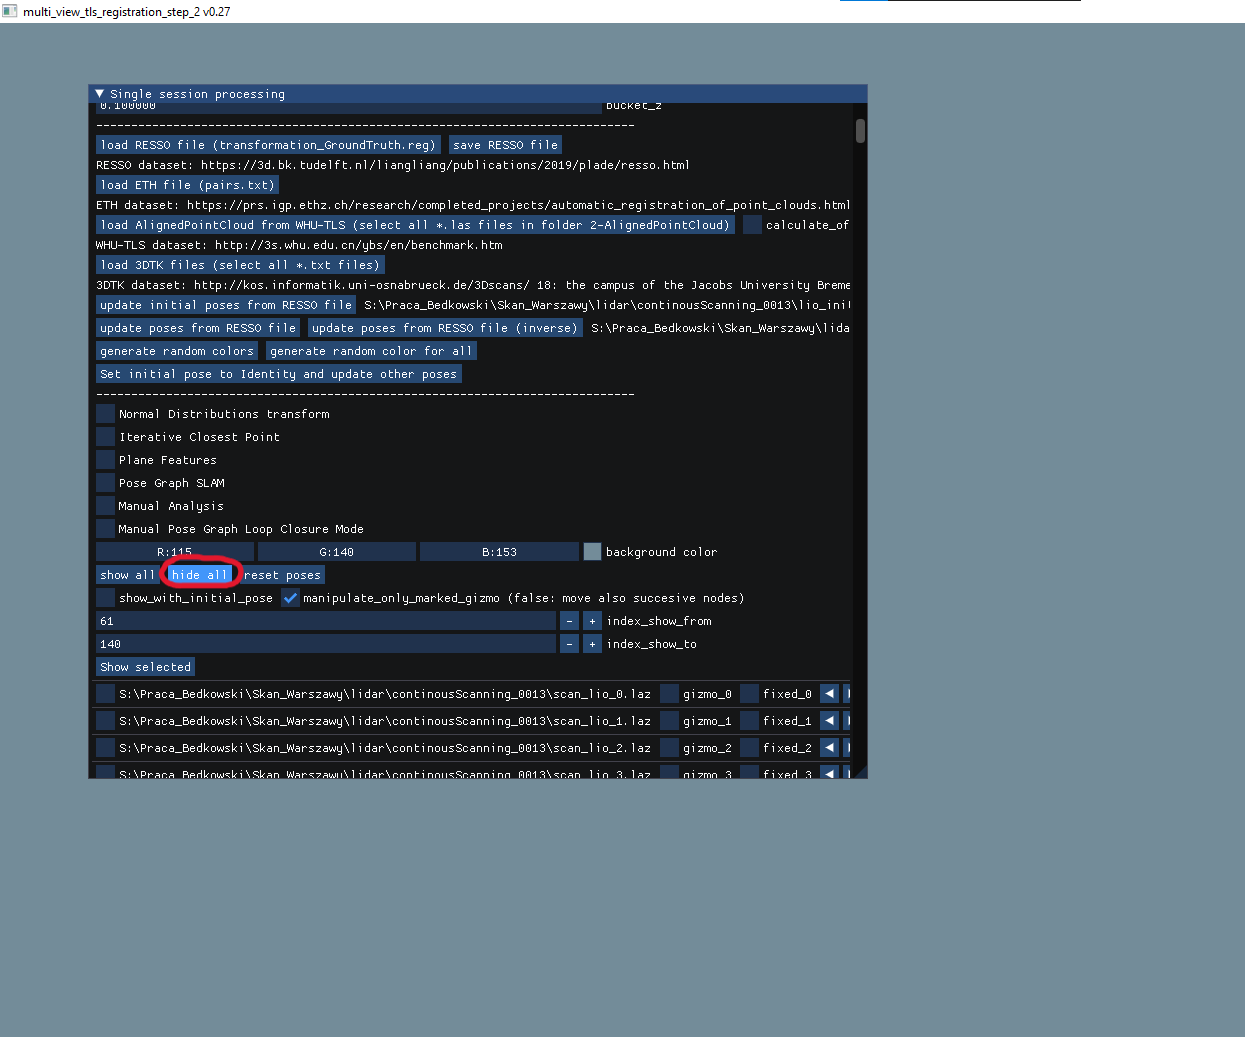
\includegraphics[width=\textwidth]{Cut_session2.png}
	\caption{Scroll down to list of scans and click hide all.}
	\label{fig:21}
\end{figure}

\begin{figure}[H]
	\centering
	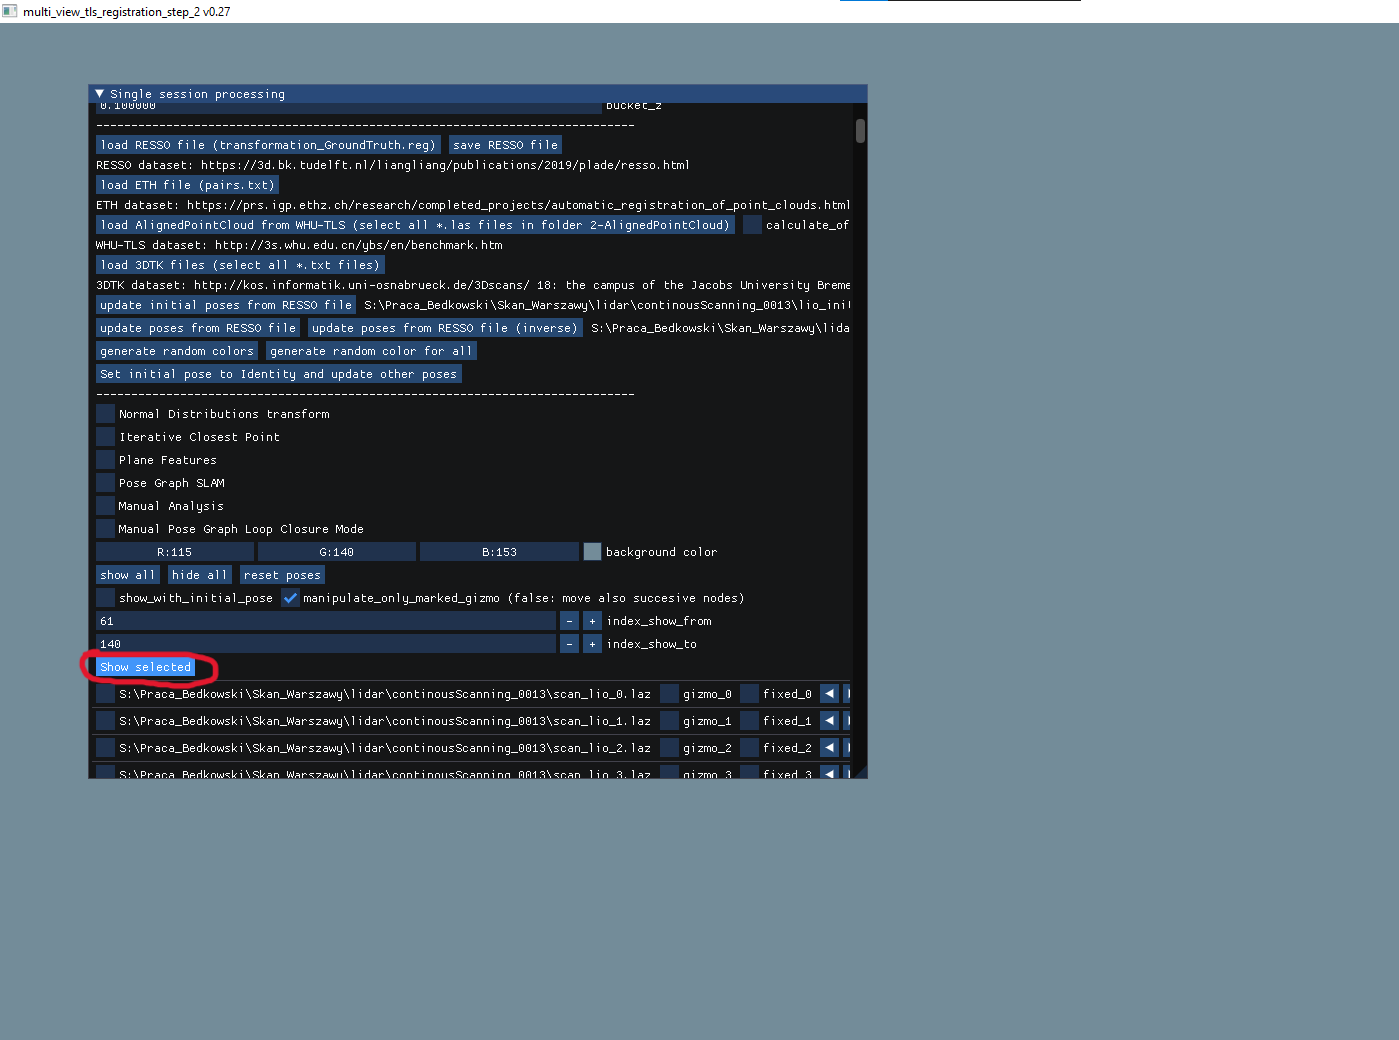
\includegraphics[width=\textwidth]{Cut_session3.png}
	\caption{Write indexes of the beginning scan and ending scan then click Show selected. The scans between the indicated ones will appear. This step may be repeated to build a session form many, separated fragments.}
	\label{fig:22}
\end{figure}

\begin{figure}[H]
	\centering
	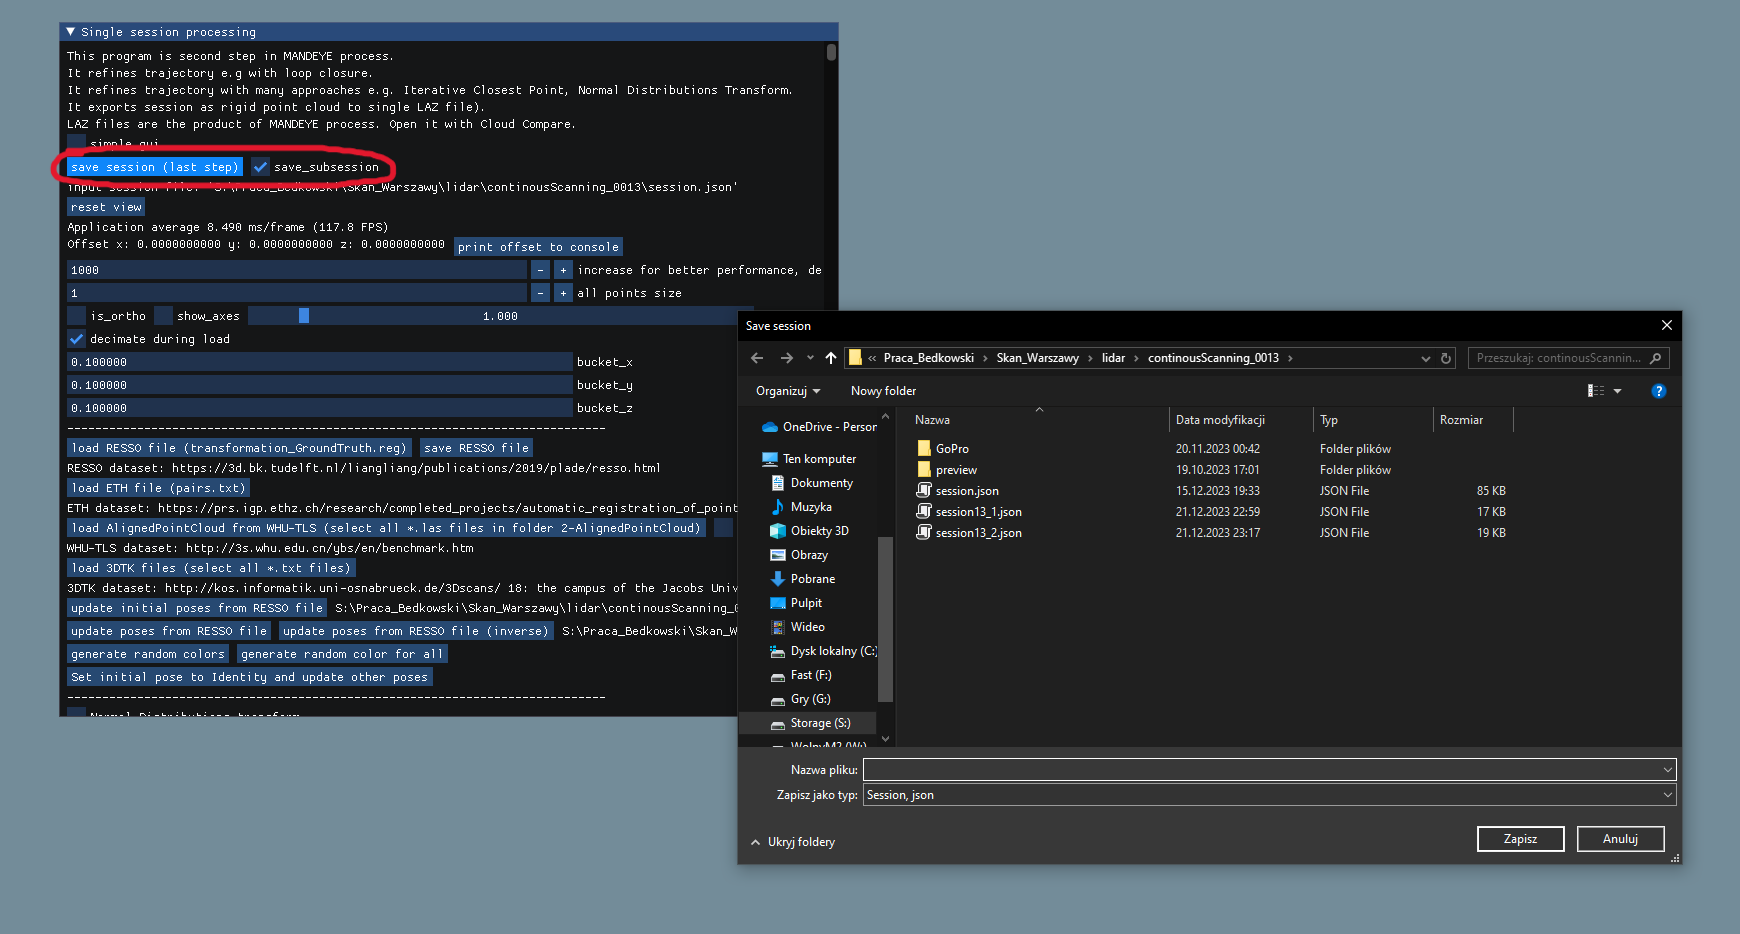
\includegraphics[width=\textwidth]{Cut_session4.png}
	\caption{With desired scans selected scroll up, select save subsession and click save session. Save the session to a new .json session file.}
	\label{fig:23}
\end{figure}

\begin{figure}[H]
	\centering
	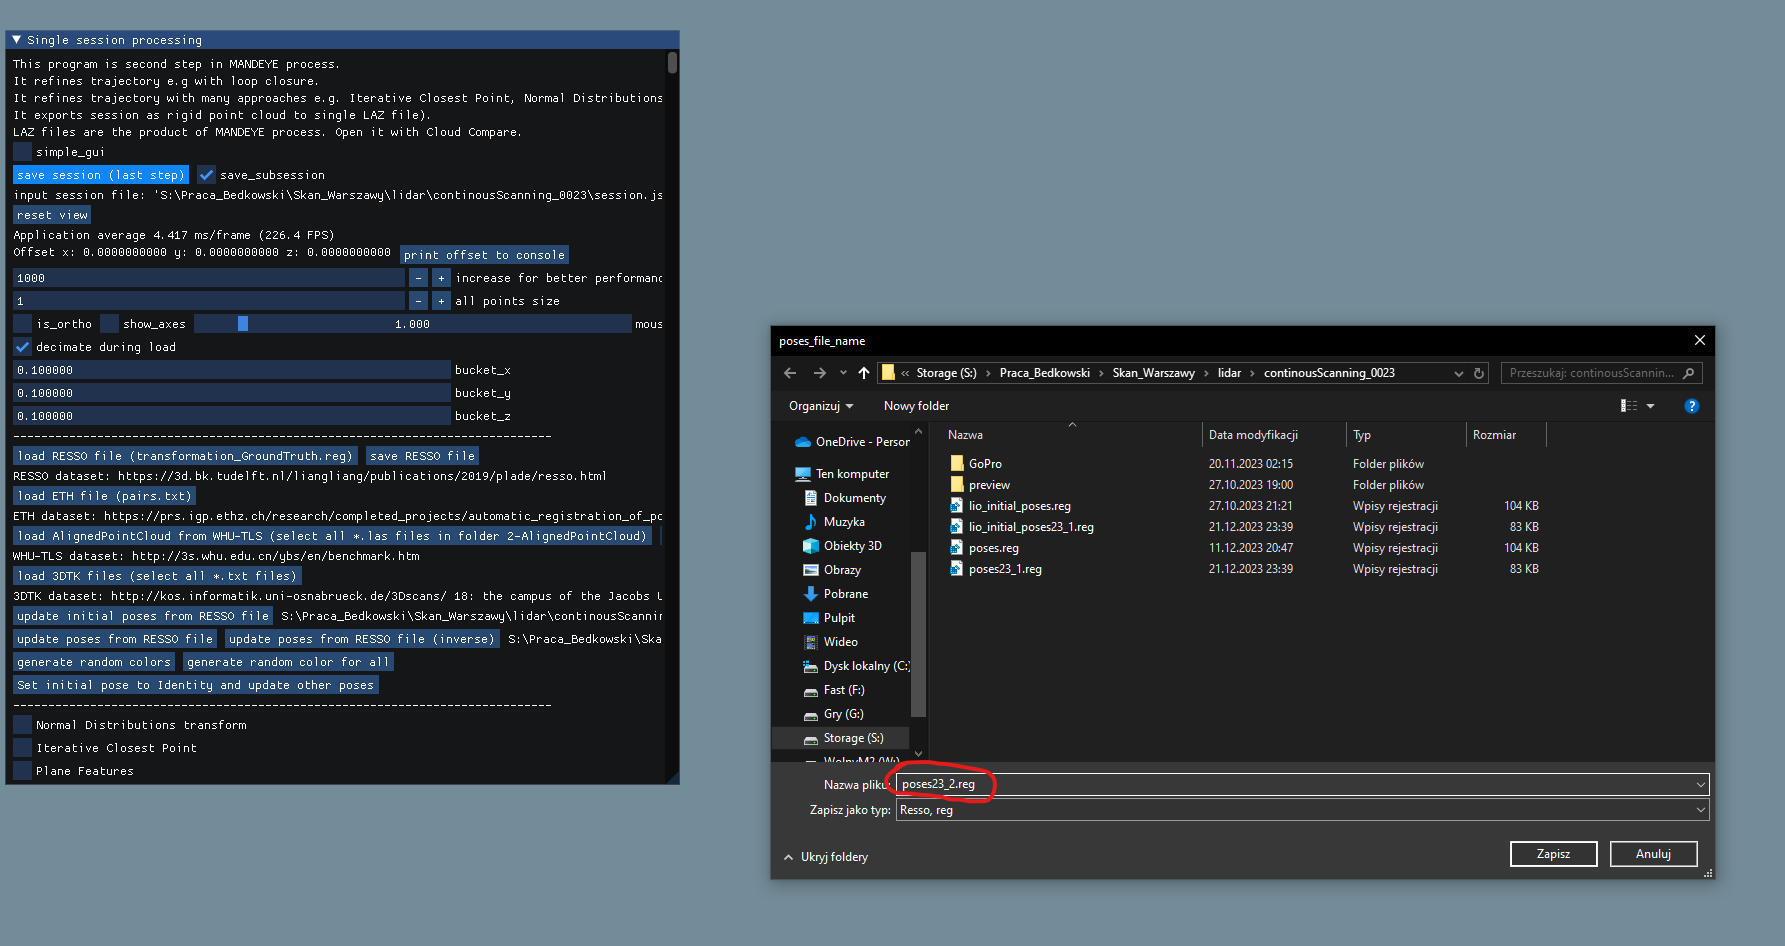
\includegraphics[width=\textwidth]{Cut_session5.png}
	\caption{After a .json session file is saved, proceed with creating new resso .reg file and saving poses to it.}
	\label{fig:24}
\end{figure}

\begin{figure}[H]
	\centering
	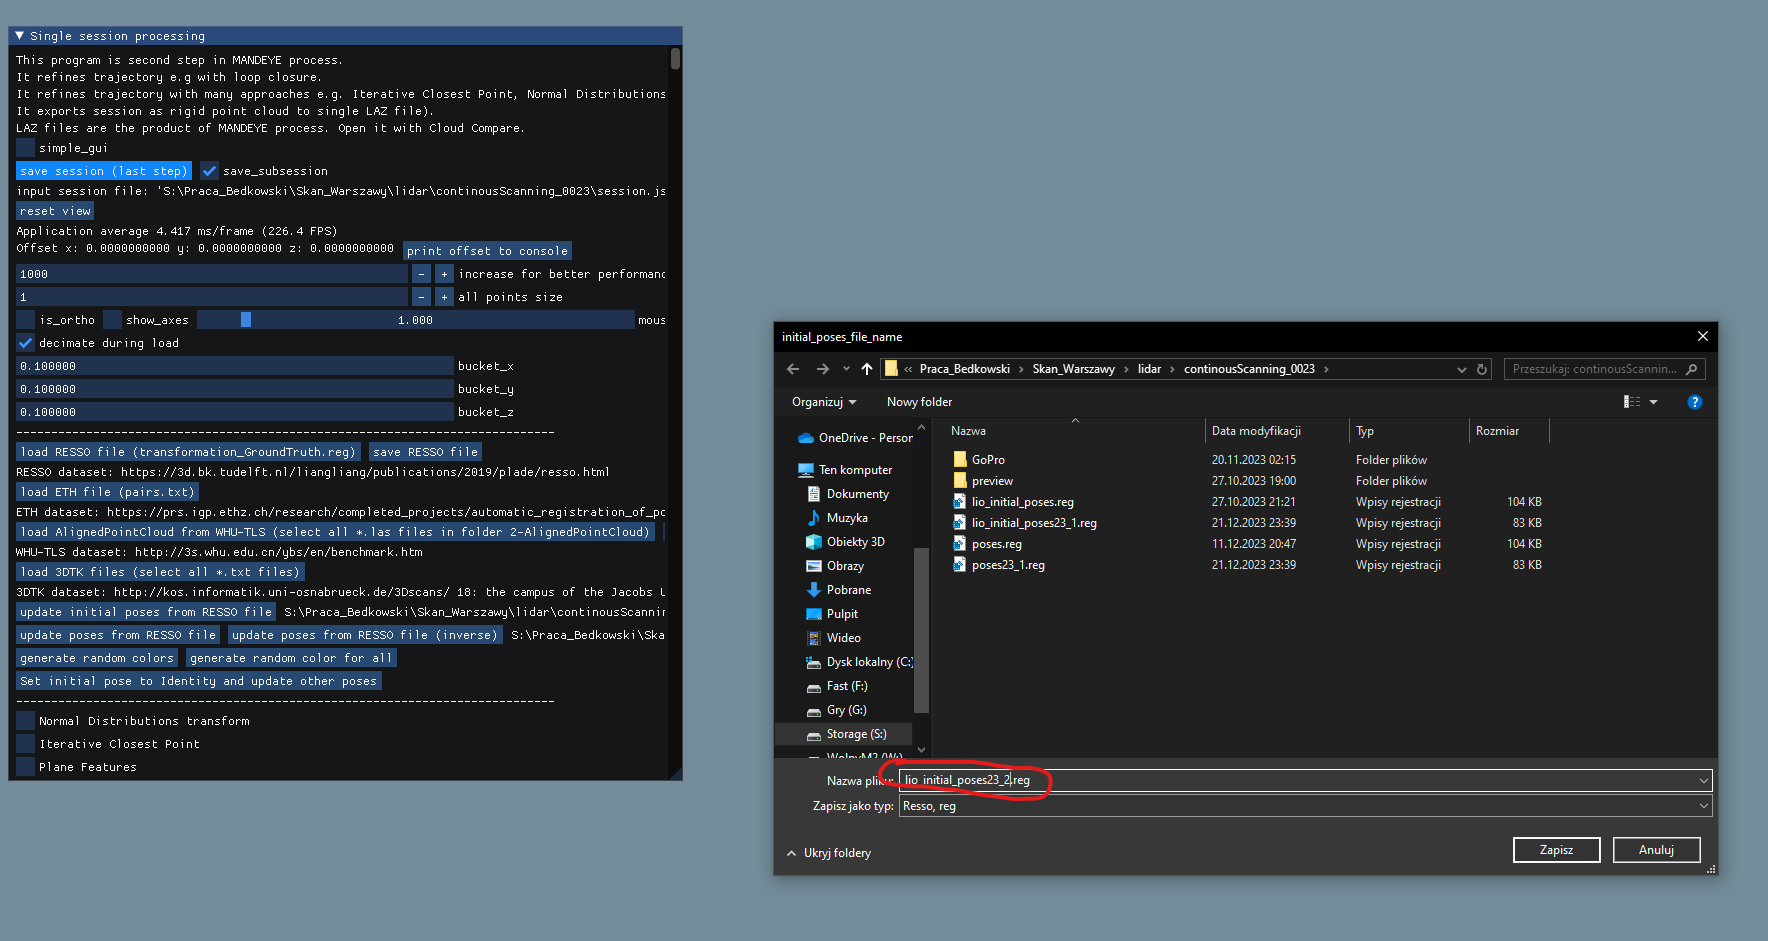
\includegraphics[width=\textwidth]{Cut_session6.png}
	\caption{Do the same as in previous step with initial poses file - create new file and save it.}
	\label{fig:25}
\end{figure}

\section{Step 3}
\begin{figure}[H]
	\centering
	\includegraphics[width=\textwidth]{20.png}
	\caption{Add sessions that you want to align.}
	\label{fig:26}
\end{figure}

\begin{figure}[H]
	\centering
	\includegraphics[width=\textwidth]{21.png}
	\caption{Choose session.json files - effects of the lidar odometry step.}
	\label{fig:27}
\end{figure}

\begin{figure}[H]
	\centering
	\includegraphics[width=\textwidth]{22.png}
	\caption{Click load sessions button and wait for the chosen sessions to load.}
	\label{fig:28}
\end{figure}

\begin{figure}[H]
	\centering
	\includegraphics[width=\textwidth]{23.png}
	\caption{When all of the sessions have loaded activate Manual Pose Graph Loop Closure Mode. If more than 2 sessions were loaded, deactivate sessions till two of them remain. After that the button should appear.}
	\label{fig:29}
\end{figure}

\begin{figure}[H]
	\centering
	\includegraphics[width=\textwidth]{24.png}
	\caption{Choose 2 individual scans of the same area, one from the first session, other from the second session and click add edge.}
	\label{fig:30}
\end{figure}

\begin{figure}[H]
	\centering
	\includegraphics[width=\textwidth]{25.png}
	\caption{Click manipulate active edge, then gizmo and as in \hyperref[fig:15]{the step 2} align scans as precisely as possible and then repeatedly use ICP till nothing changes.}
	\label{fig:31}
\end{figure}

\begin{figure}[H]
	\centering
	\includegraphics[width=\textwidth]{26.png}
	\caption{After aligning scans turn off Manual Pose Graph Loop Closure Mode, click Optimize and if everything is ok then click Save results. Should anything go wrong and sessions haven't orientated as planned just use Revert button. Repeat steps 3.13-3.15 until two sessions are aligned with a satisfying effect.}
	\label{fig:32}
\end{figure}

\begin{figure}[H]
	\centering
	\includegraphics[width=\textwidth]{27.png}
	\caption{At the end or in the middle of work you can save your project to .json file, which can be loaded next time multi session registration step 3 is used.}
	\label{fig:33}
\end{figure}

\chapter{Georeferencing}
\section{Georeferencing with point cloud}

It is possible to set session as ground truth.
Thus, optimization process (Pose GRAPH SLAM) will not change its poses.
Other sessions can be aligned against ground truth session by adding edges.

\begin{figure}[H]
	\centering
	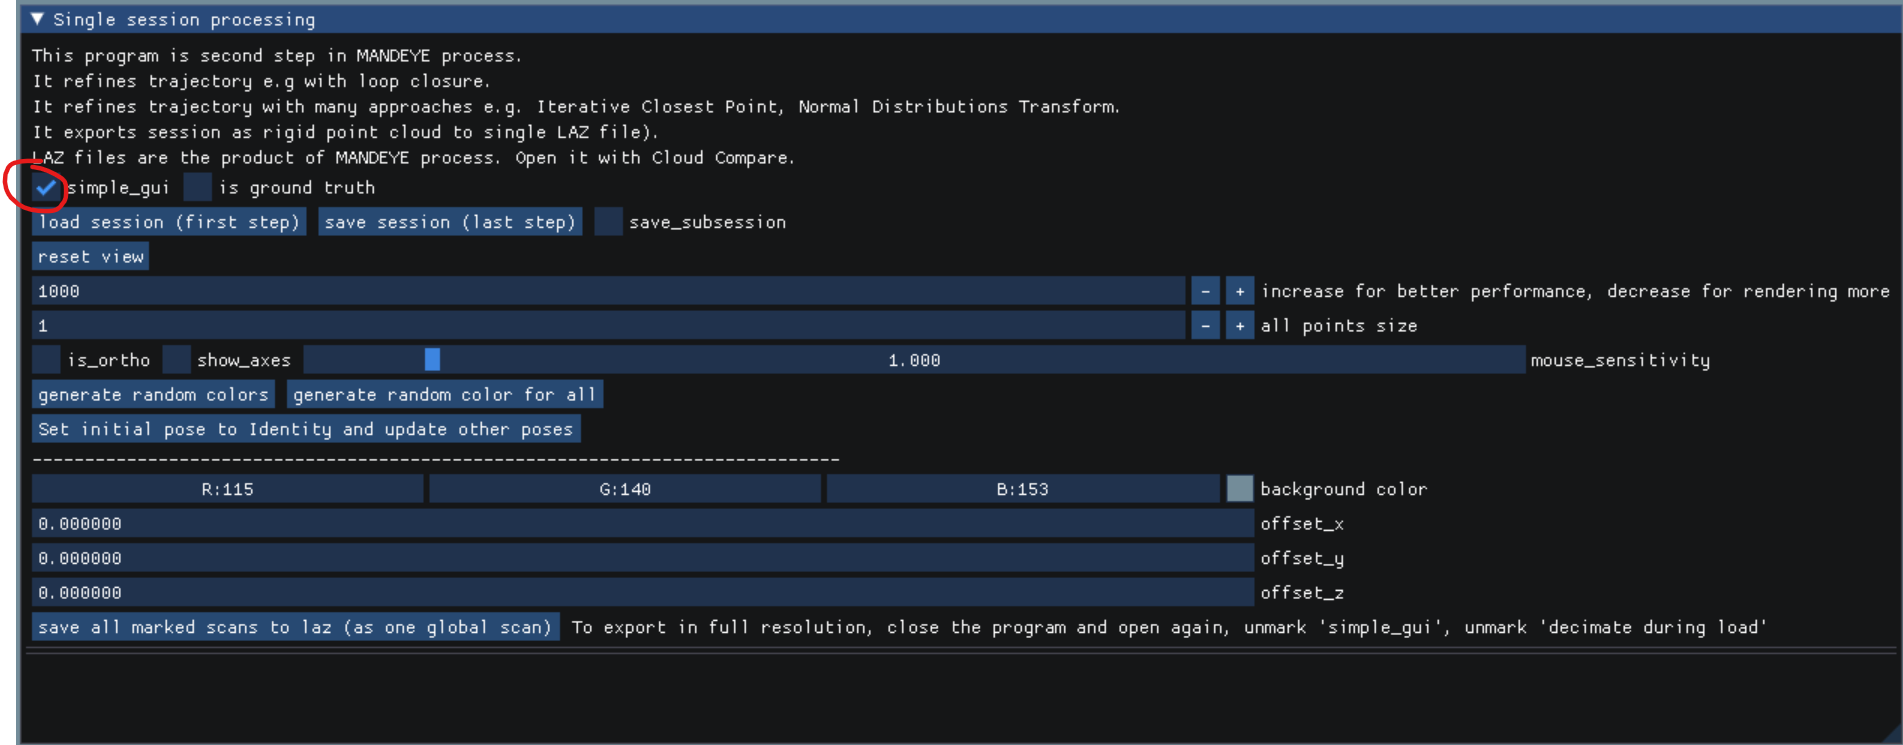
\includegraphics[width=\textwidth]{g1.png}
	\caption{Use multi view tls registration step2 program to open TLS files.}
	\label{fig:g1}
\end{figure}

\begin{figure}[H]
	\centering
	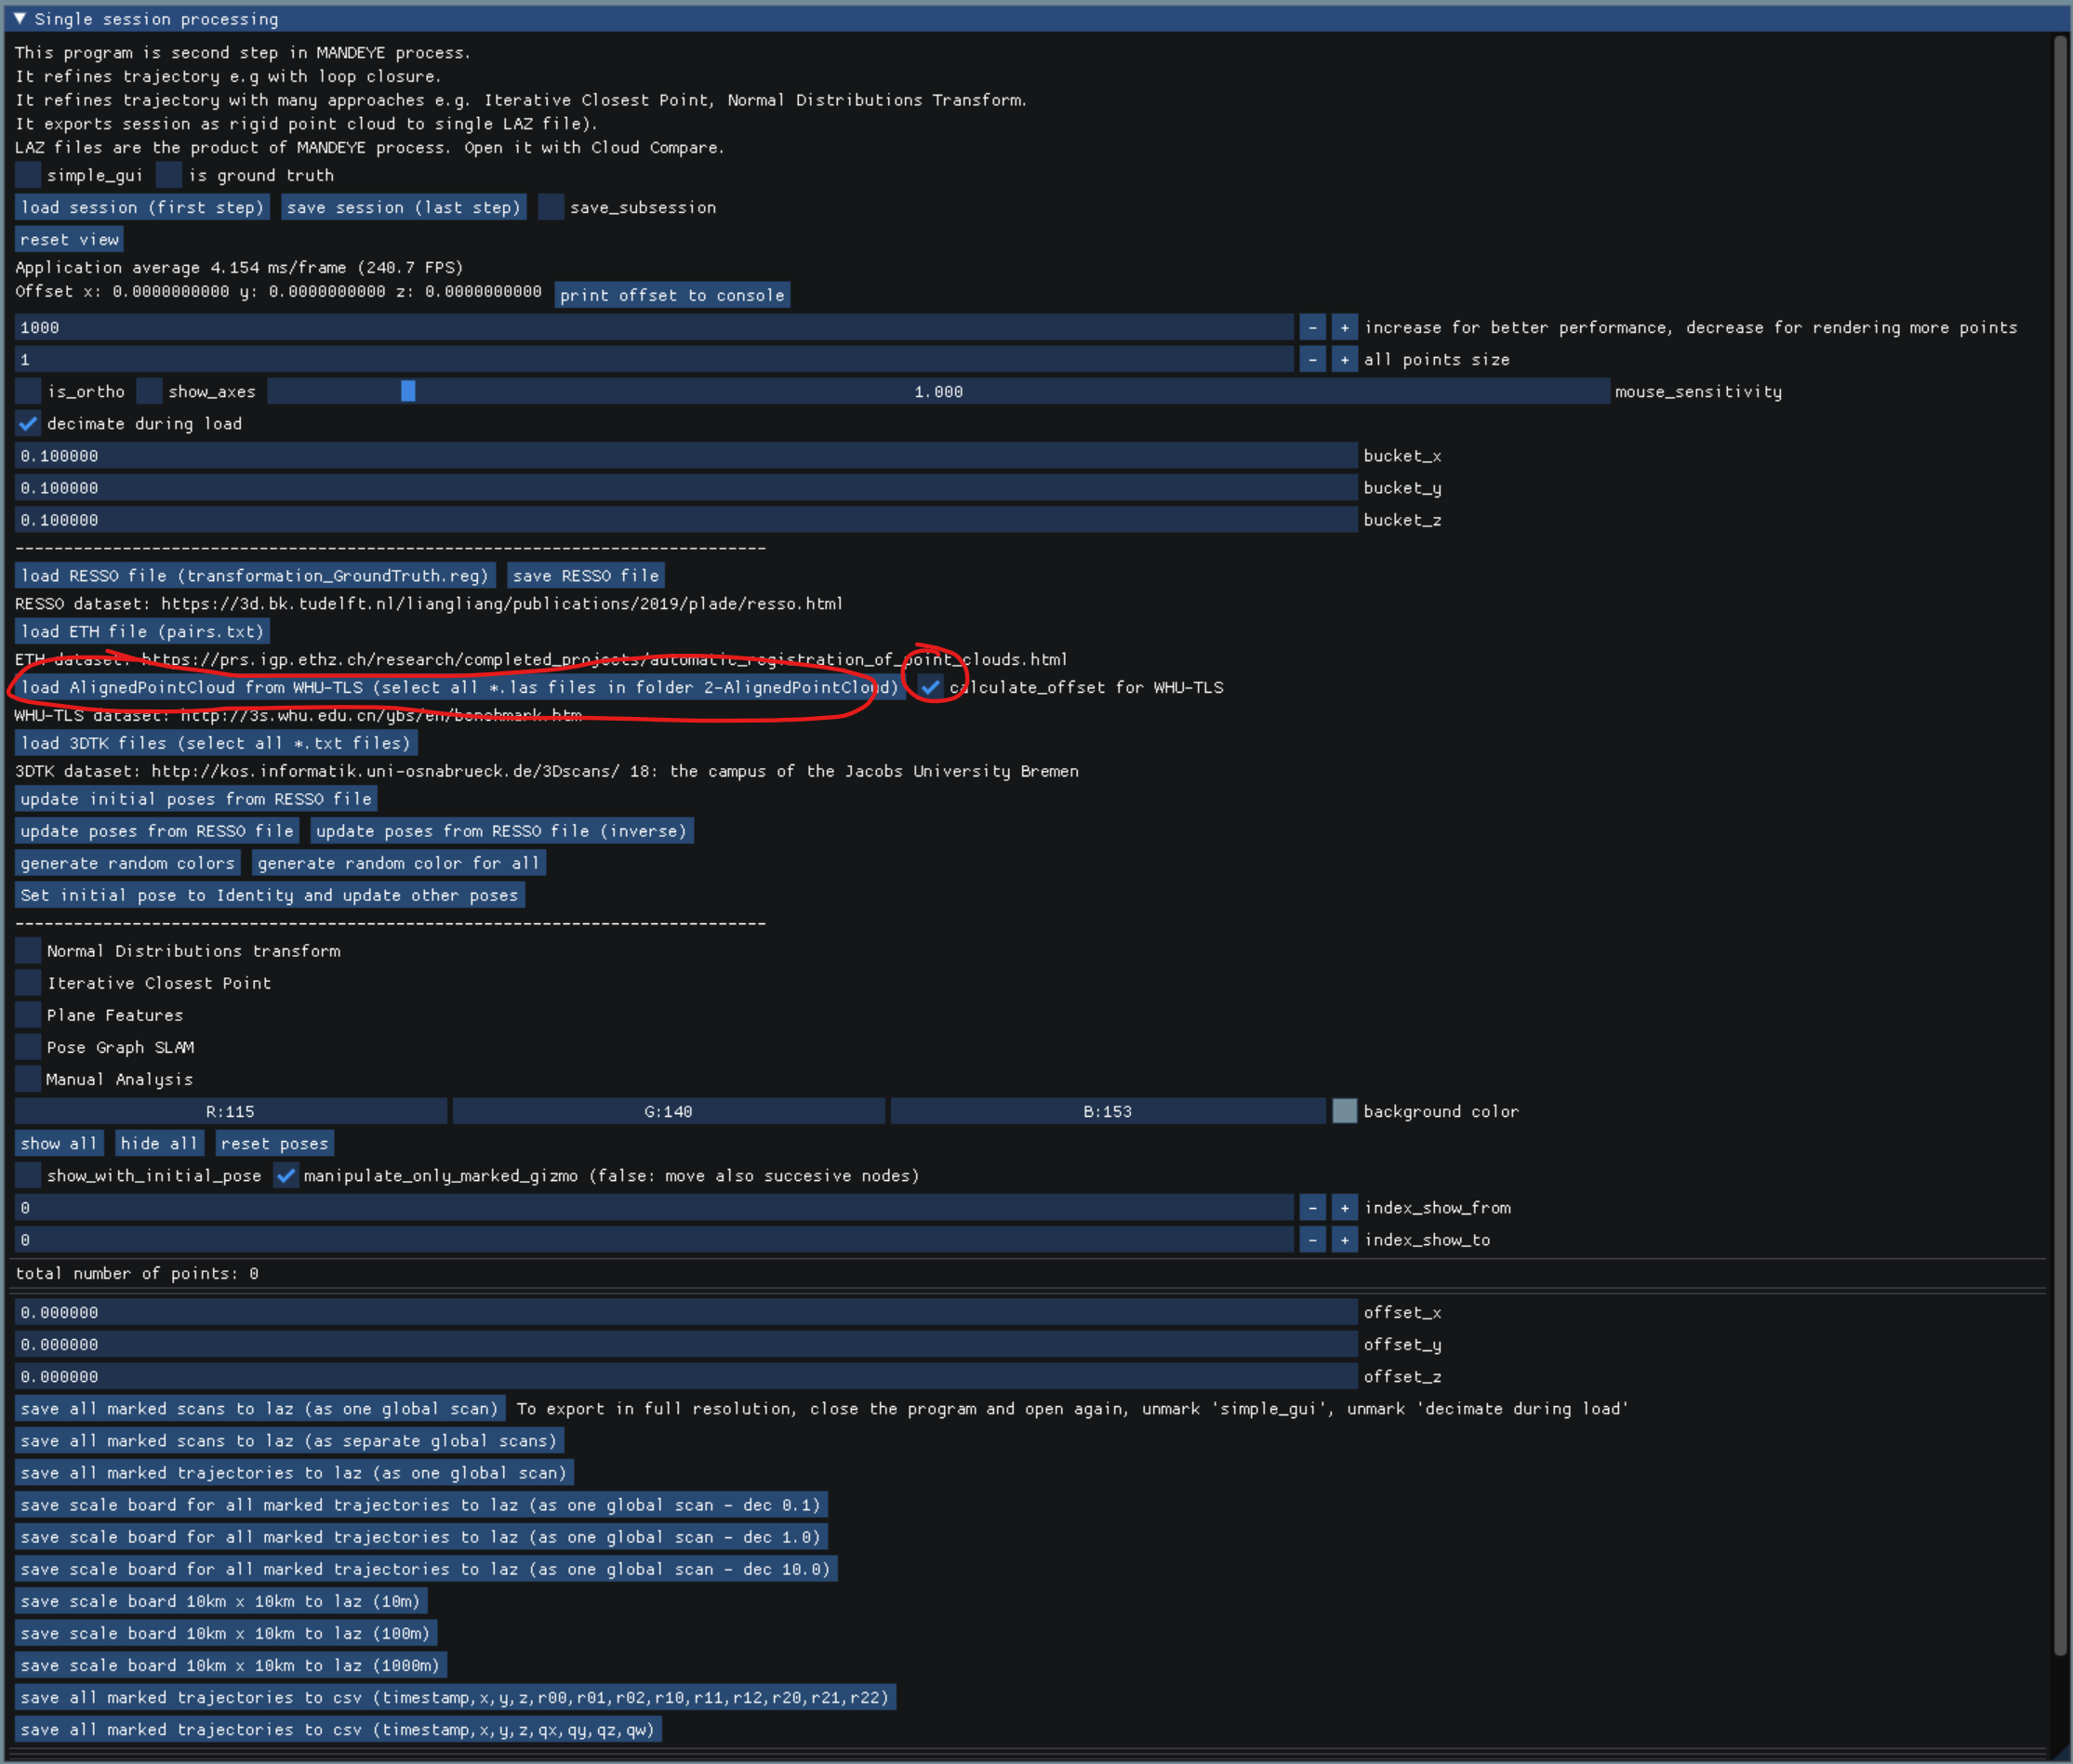
\includegraphics[width=\textwidth]{g2.png}
	\caption{Mark calculate offset for WHU-TLS, load AlignedPointCloud from WHU-TLS (select all *.las/laz files in folder)}
	\label{fig:g2}
\end{figure}

\begin{figure}[H]
	\centering
	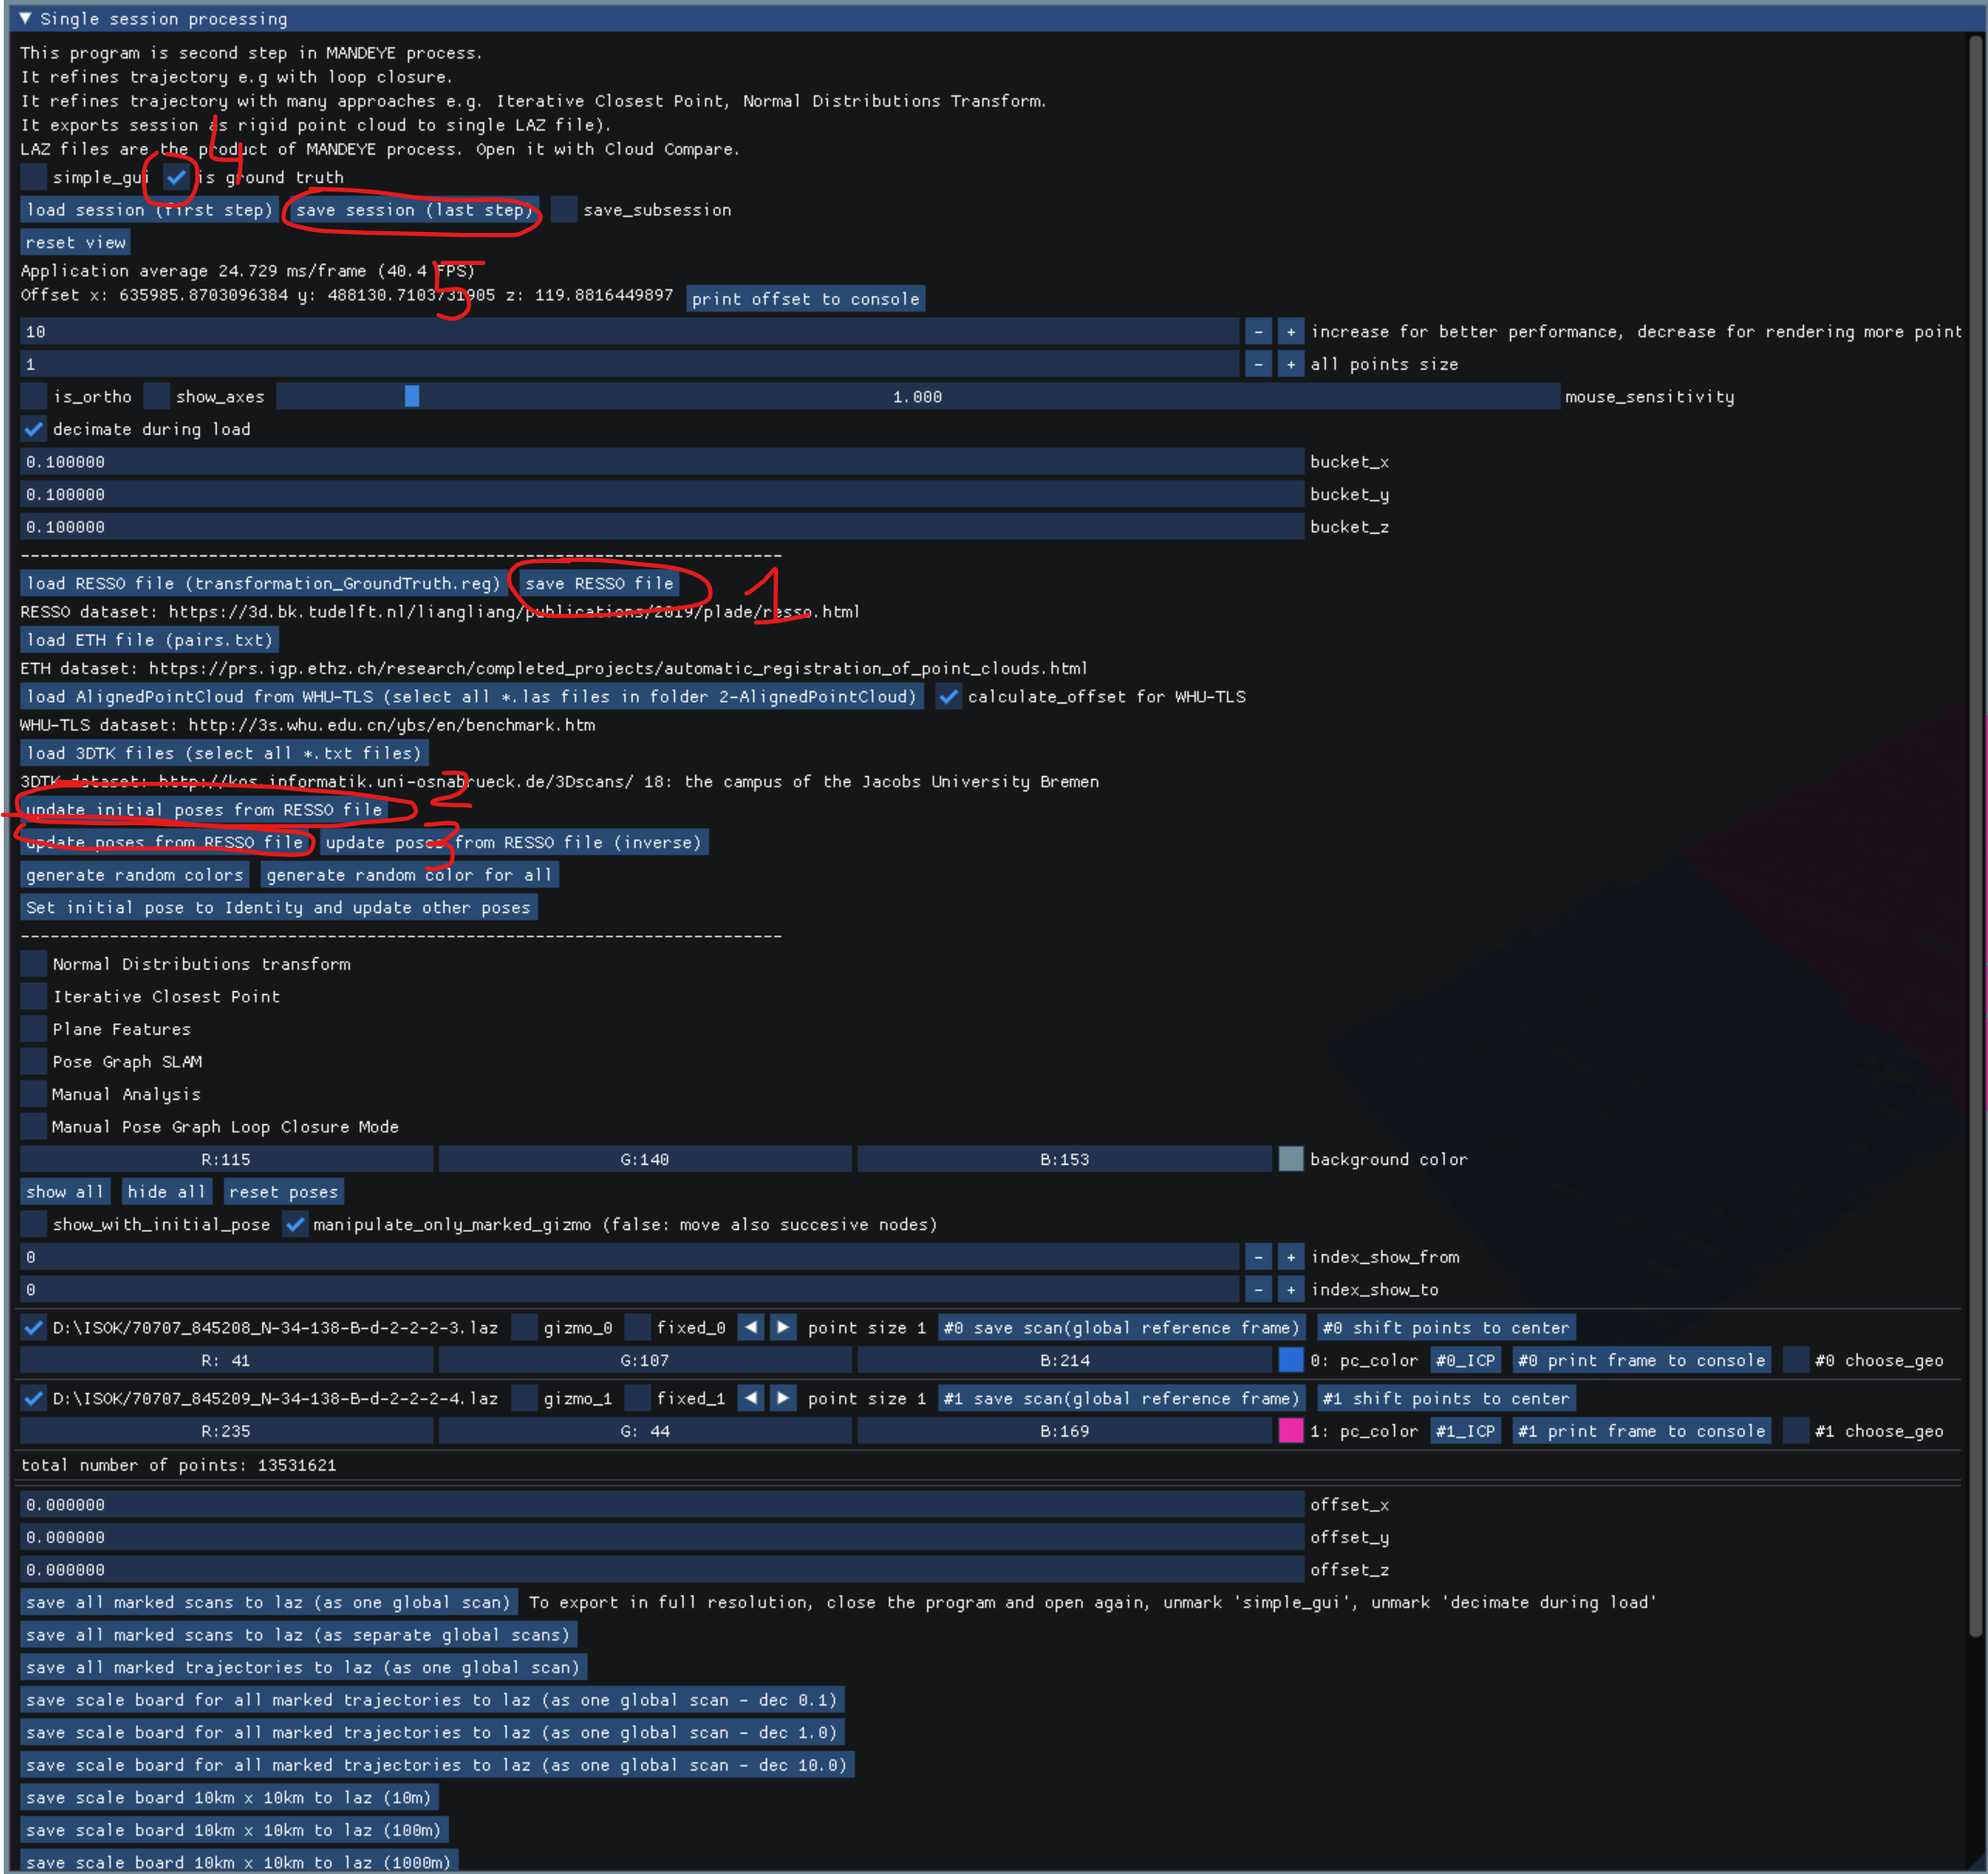
\includegraphics[width=\textwidth]{g3.png}
	\caption{1: save RESSO file, 2: update initial poses from RESSO file (select file from 1), 3: update poses from RESSO file (select file from 1), 4: set checkbox is ground truth, 5: save session.}
	\label{fig:g3}
\end{figure}

\section{Georeferencing with WGS84toCartesian}
\label{Georeferencing_with_WGS84toCartesian}
It uses \url{https://github.com/chrberger/WGS84toCartesian/tree/master} WGS84toCartesian.
It is a small and efficient library written in modern C++ library to convert WGS84 latitude/longitude positions to/from Cartesian positions using Mercator projection.
If You have MANDEYE with GNSS receiver, then it saves data in gnssXXXX.gnss files.
This is ASCII file with\\
---\\
timestamp lat lon alt hdop satelites-tracked height age time fix-quality\\
---\
\begin{figure}[H]
	\centering
	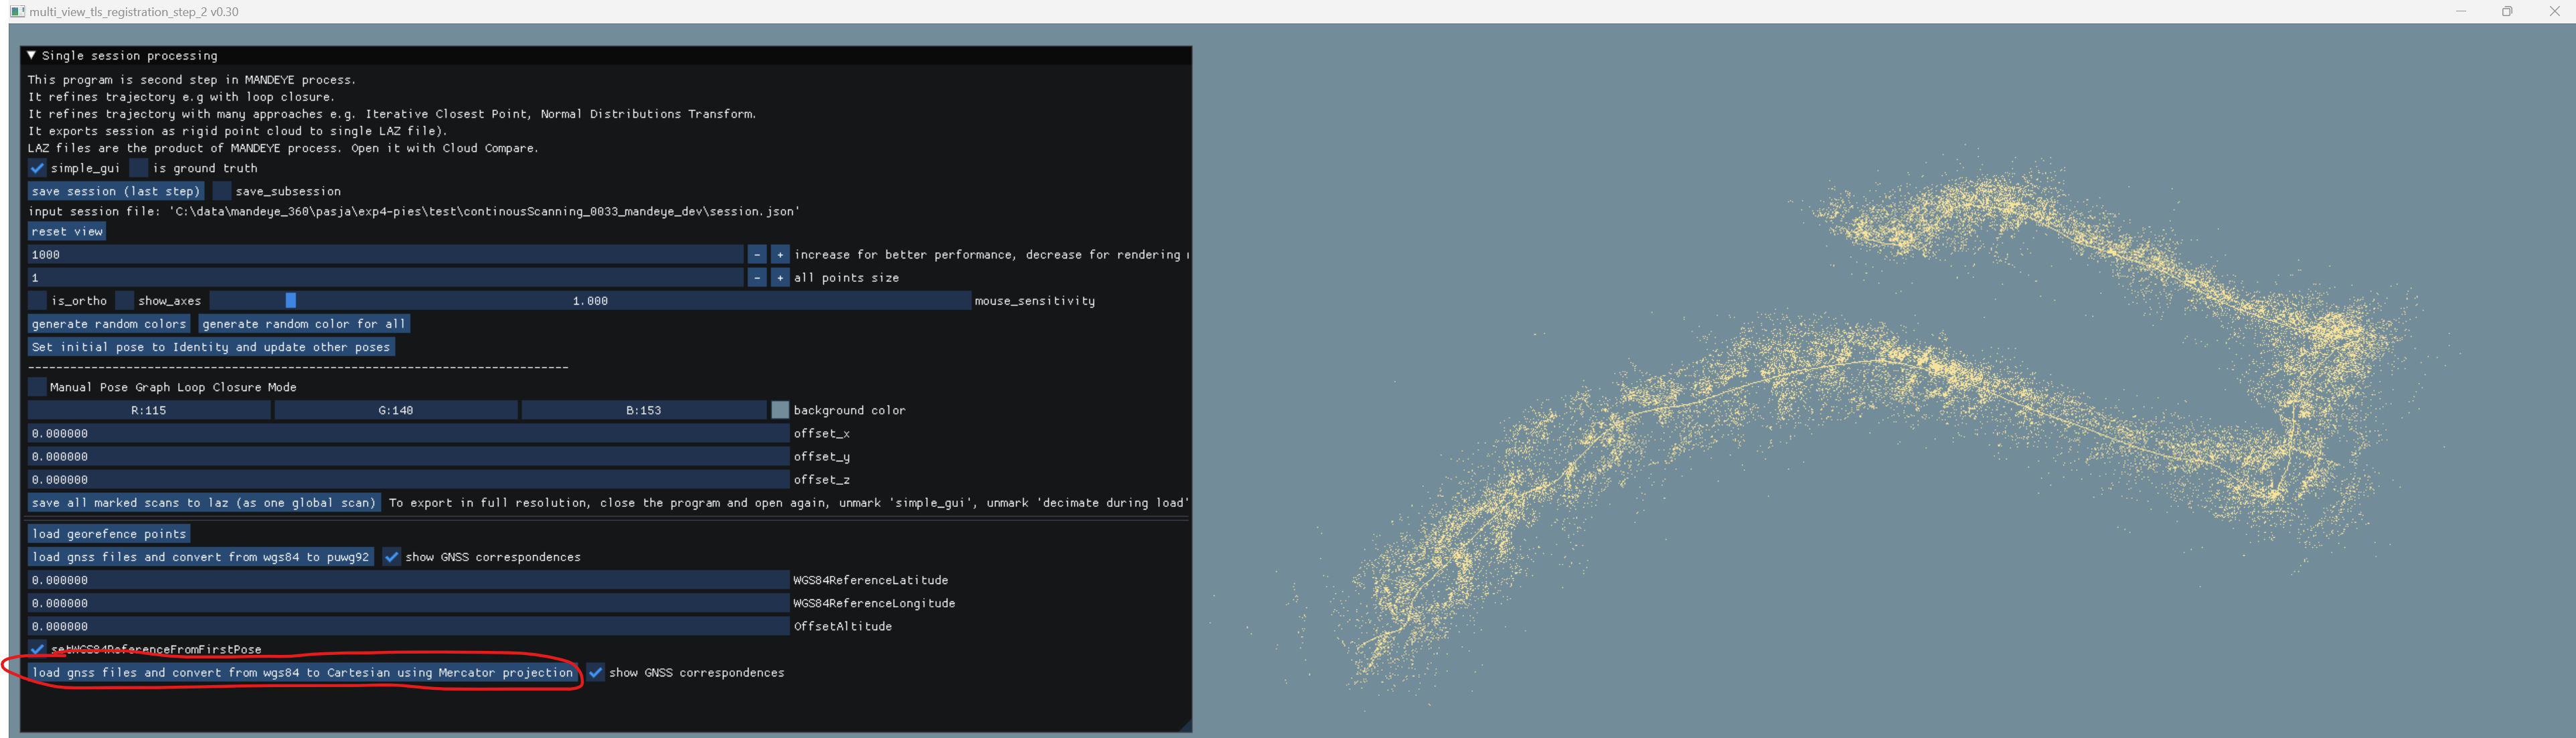
\includegraphics[width=\textwidth]{geo0.png}
	\caption{Georeferencing step 1: load gnss files and convert from wgs84 to Cartesian using Mercator projection.}
	\label{fig:geo0}
\end{figure}

\begin{figure}[H]
	\centering
	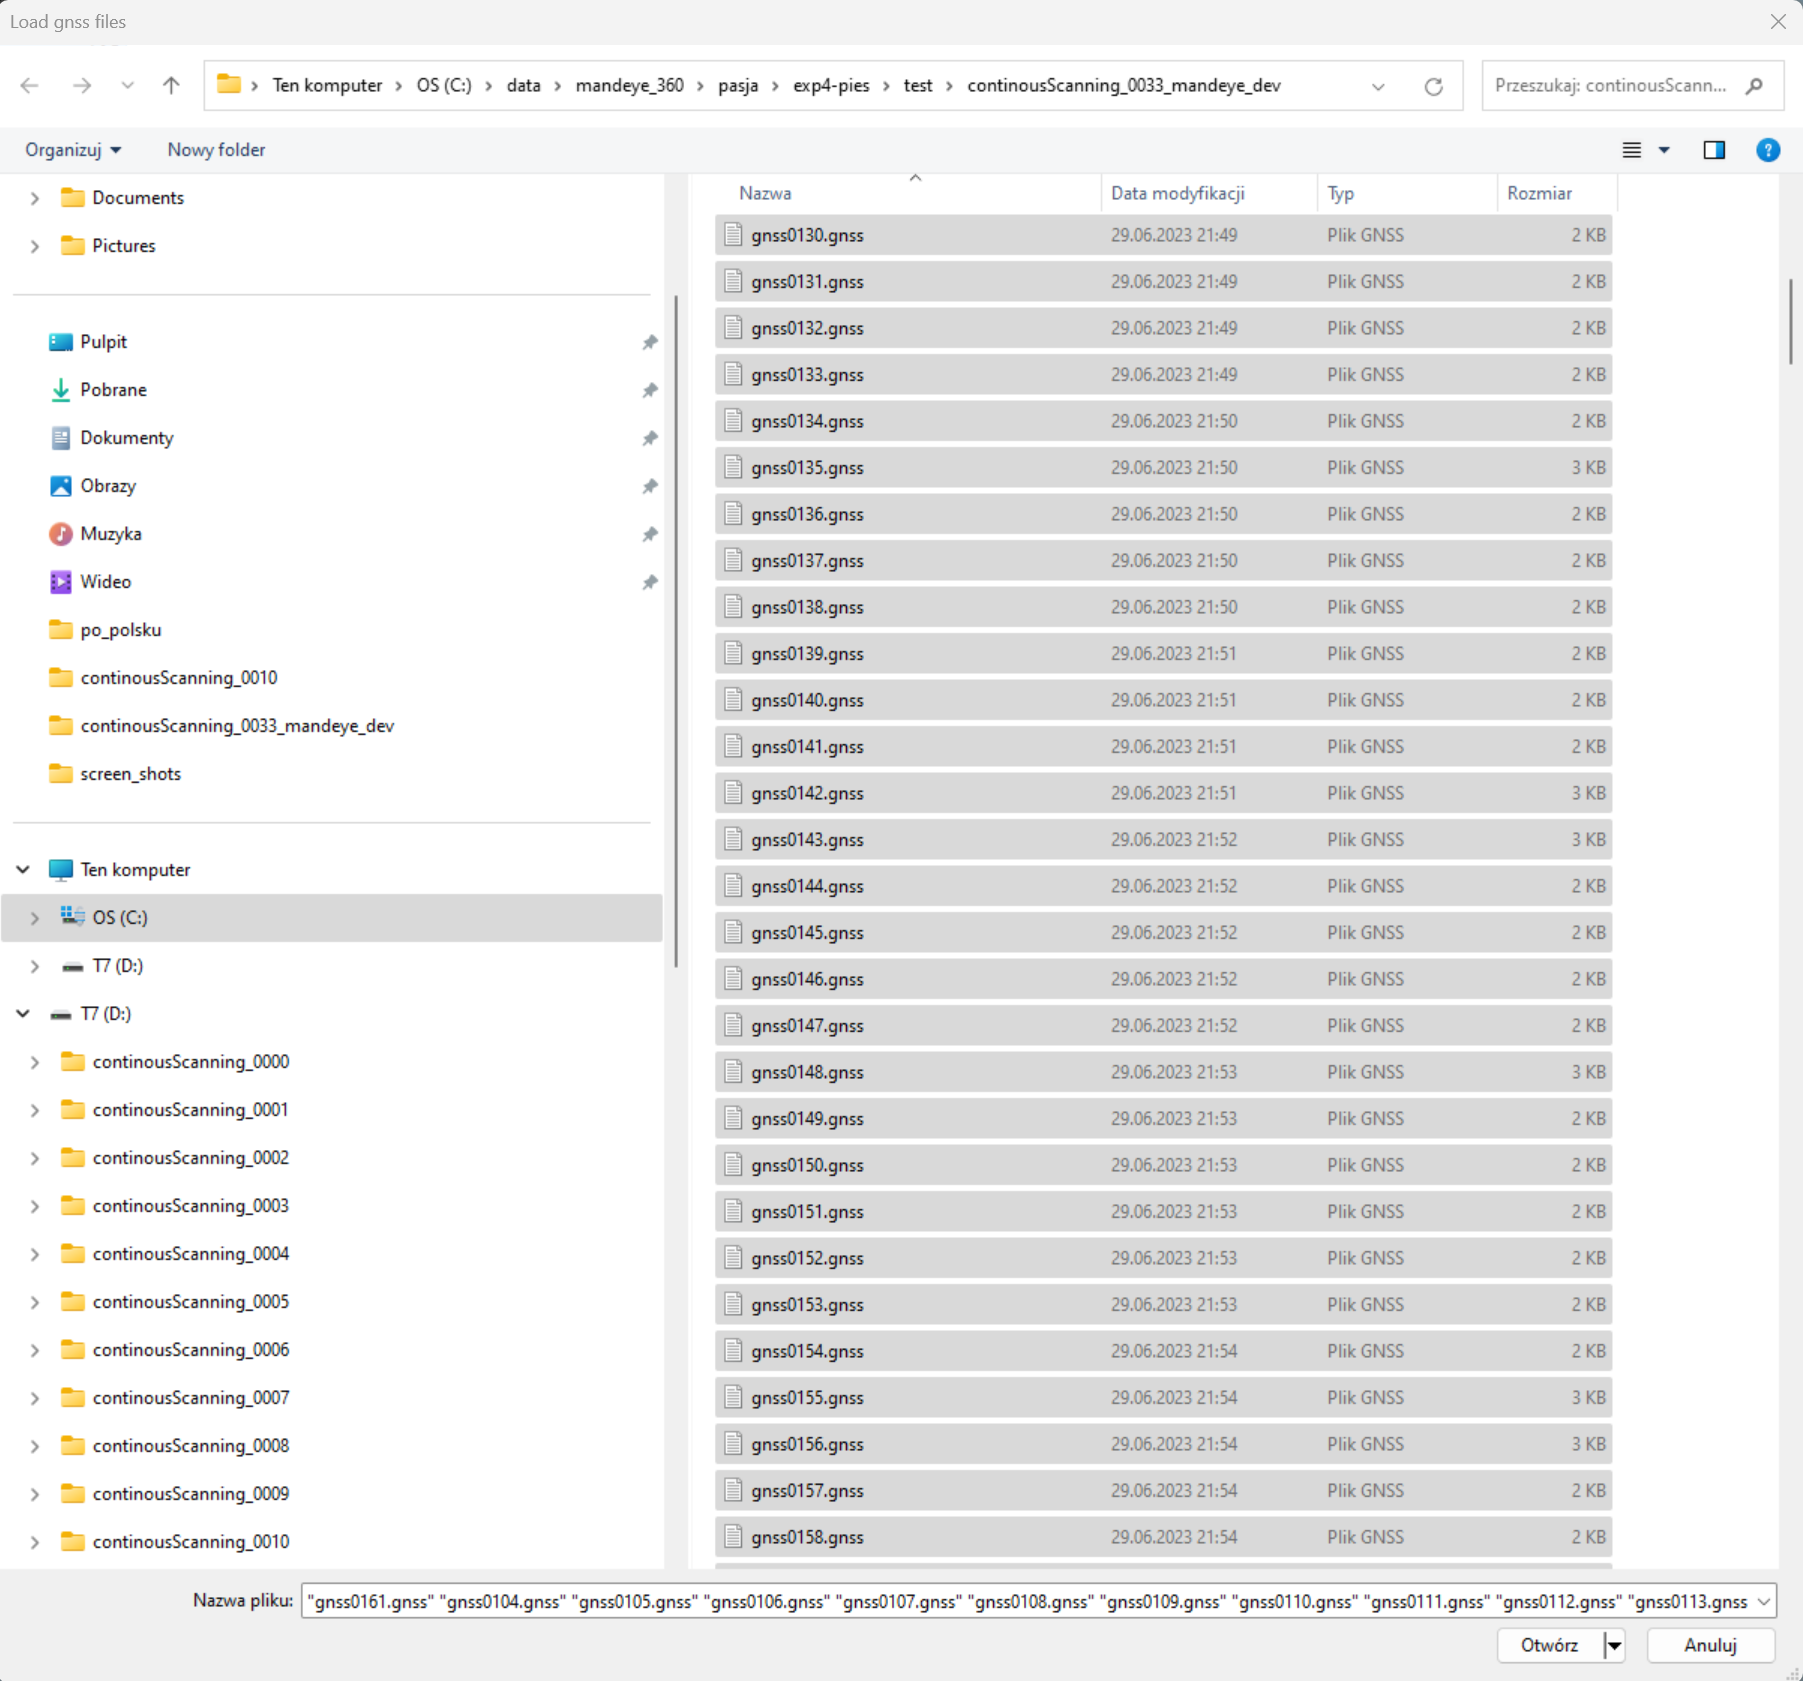
\includegraphics[width=\textwidth]{geo1.png}
	\caption{Georeferencing step 2: mark all gnss files and load.}
	\label{fig:geo1}
\end{figure}

\begin{figure}[H]
	\centering
	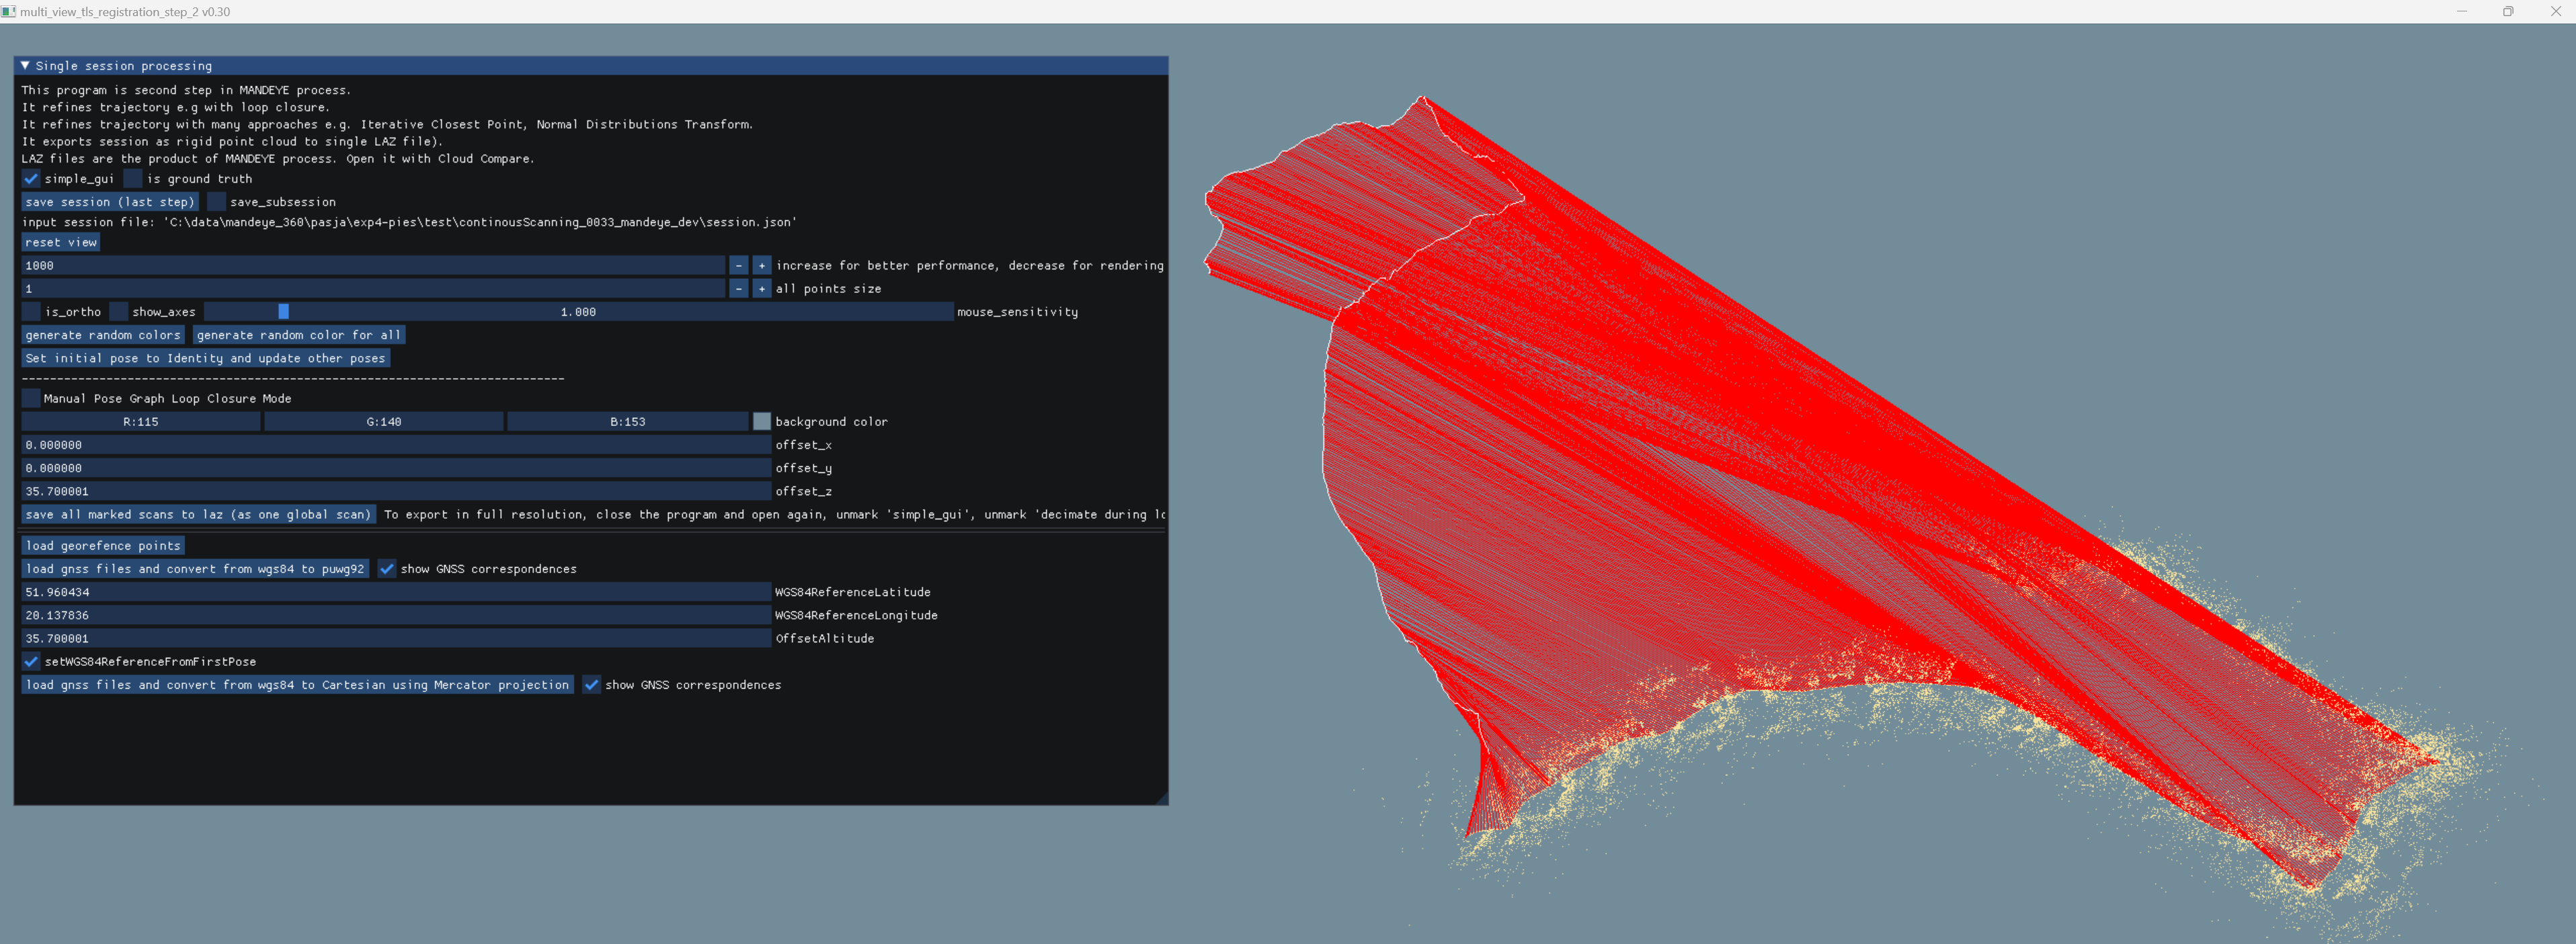
\includegraphics[width=\textwidth]{geo2.png}
	\caption{Georeferencing step 3: check/uncheck 'show GNSS correspondences' to see gnss-poses correspondences. Remark: You can use gizmo for manual initial trajectory to GNSS alignment.}
	\label{fig:geo2}
\end{figure}

\begin{figure}[H]
	\centering
	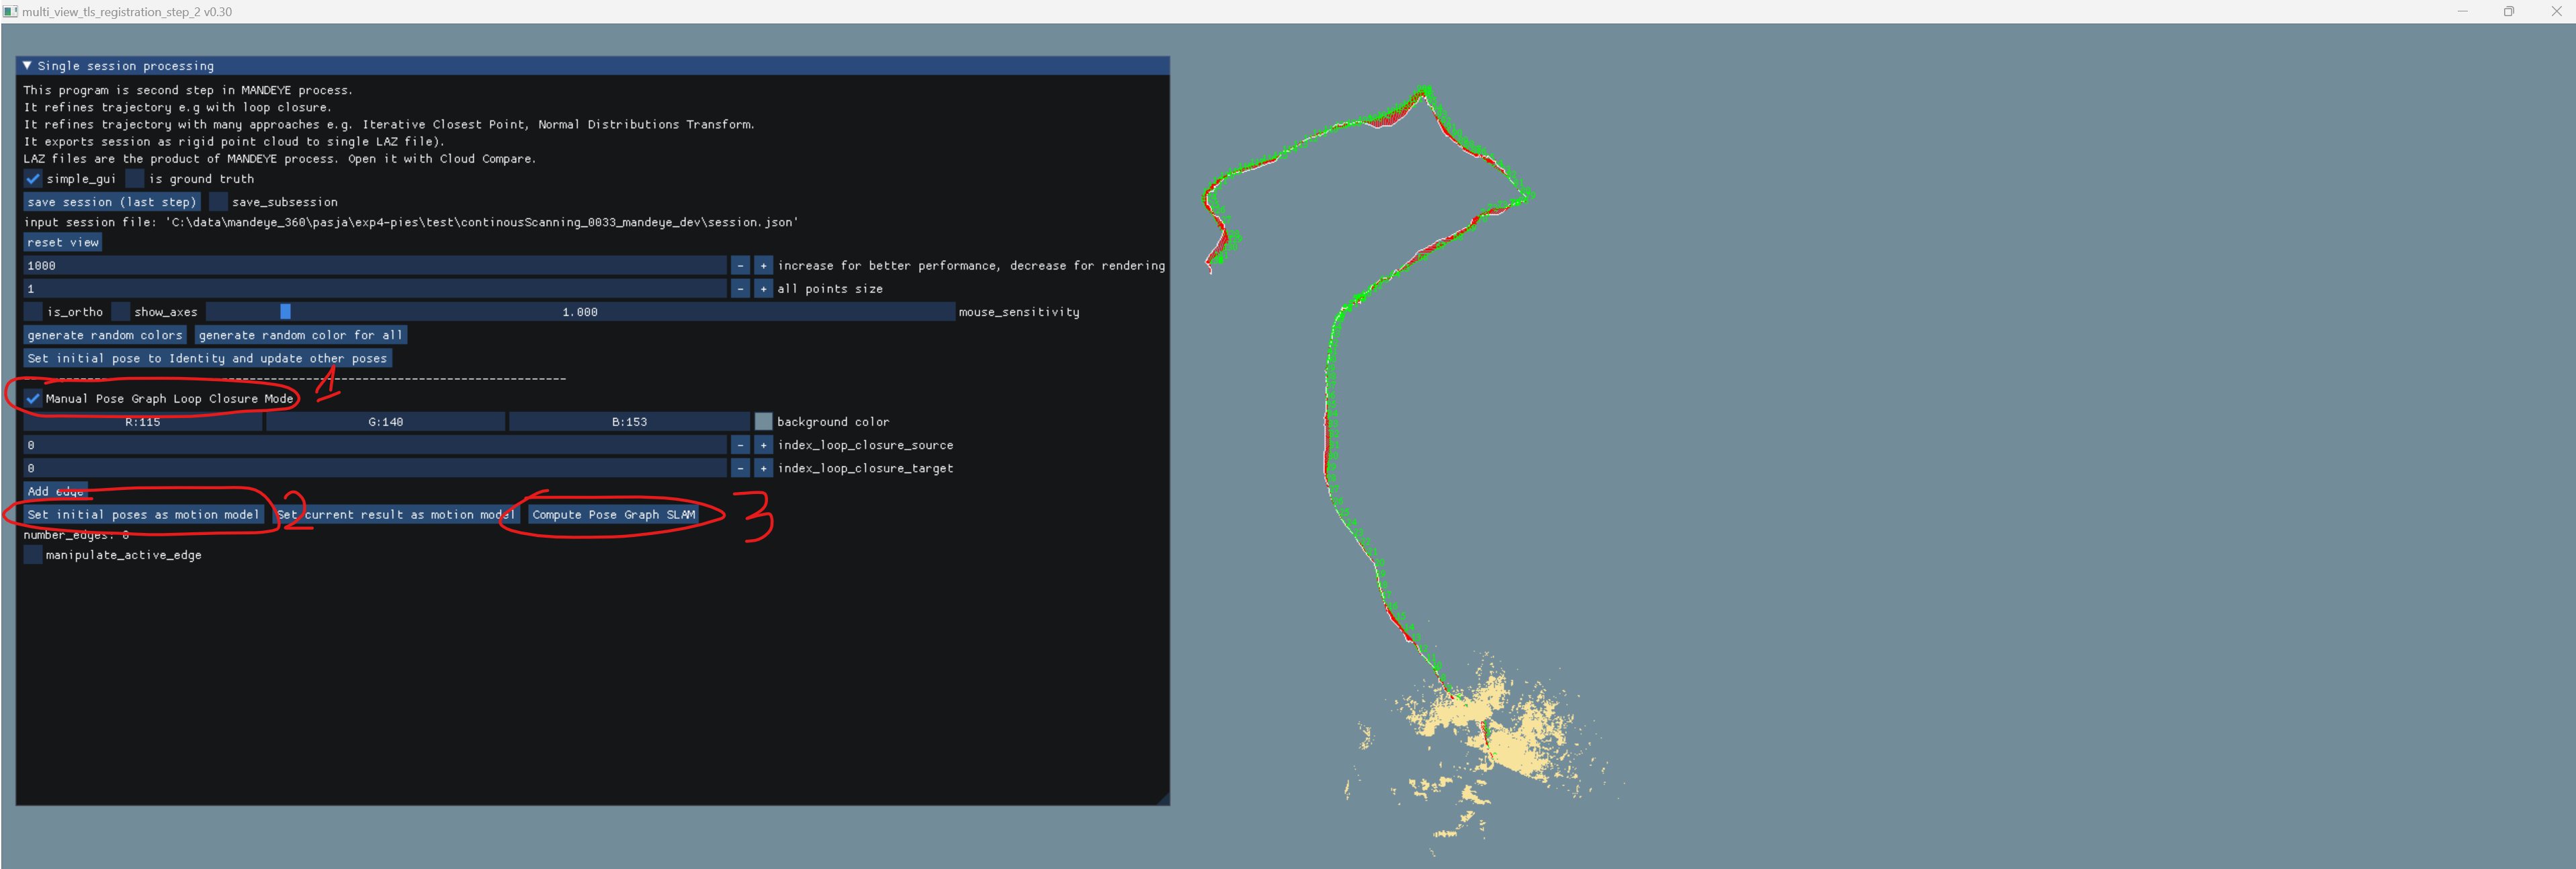
\includegraphics[width=\textwidth]{geo3.png}
	\caption{Georeferencing step 4: Check Manual Pose Graph Loop Closure Mode, then set initial poses as motion model, then Compute Pose Graph SLAM.}
	\label{fig:geo3}
\end{figure}

\chapter{Questions from end users}

\textbf{Do you have recommendations on how to best record data?} \\
I recommend stop/scan mode for most accurate mapping.
Continuous mapping is for increase the time of the survey.  \\
\textbf{How much distance can be between two consecutive start/stop acquisitions?}\\
I suggest not more than 10 meters.\\
\textbf{Do they need to overlap? To which degree?}\\
Stop/scans should be overlapped at least 50\%.\\
\textbf{Continuous scanning: can the sensor change its tilt/angle during the recording phase? 
Or does it assume being in a upright position all the time?} \\
I suggest that MANDEYE  is somehow a upright position all the time. \\
\textbf{How “fast” am I allowed to move (I actually did a rather slow walk).} \\
I was tested it up to 8 km/h\\
\textbf{Can the sensor change height while recording?}\\
Yes.\\
\textbf{Why first scan is blurry?}\\
You should follow \url{https://github.com/JanuszBedkowski/mandeye_controller/blob/main/doc/manual/manual_v0_2/mandeye_dev_manual_v0_2.pdf} - section 2.2 turn on continous scanning (MANDEYE DEV/PRO)\\
\textbf{Do you have a video of operating MANDEYE DEV?}\\
I am planning launching MANDEYE YouTube channel ASAP.\\
\textbf{Why there are 2 operations of stopping the scan?}\\
MANDEYE is working within single session scheme. It means all data will be recorded to one folder. MANDEYE will make new folder after turn of turn on procedure.\\
\textbf{The usb that came with mandeye DEV has files in it, do i need to format it?}\\
If You have MANDEYE from me (januszbedkowski@gmail.com) then Release programs and manuals are on USB. Please do not format it, just use it.\\
\textbf{How much can i scan in one session?}\\
I suggest not more than 5km. It will be much easier to work with such session. Obviously long single session can be split into sub sessions, so dont worry if You make any mistake during data collection.\\




 


\backmatter
% bibliography, glossary and index would go here.

\end{document}